\section{\href{https://survey.stackoverflow.co/2023/}{Enquêtes Stackoverflow 2023}}
\label{annexe:Ruby_stats}

\subsection{Langages utilisés par les sondé.e.s cette année et ceux envisagés pour l'année suivante}

\begin{quote}
    Quels langages de programmation, de script et de balisage avez-vous utilisés de manière extensive au cours de la dernière année, et lesquels souhaitez-vous utiliser au cours de l'année à venir ? (Si vous avez à la fois travaillé avec le langage et que vous souhaitez continuer à le faire, veuillez cocher les deux cases dans cette ligne.)\footnote{\textit{Which programming, scripting, and markup languages have you done extensive development work in over the past year, and which do you want to work in over the next year? (If you both worked with the language and want to continue to do so, please check both boxes in that row.)}}
\end{quote}


    \begin{figure}[H]
    %centrer l'image
        \centering
        %commande qui permet de charger une image
        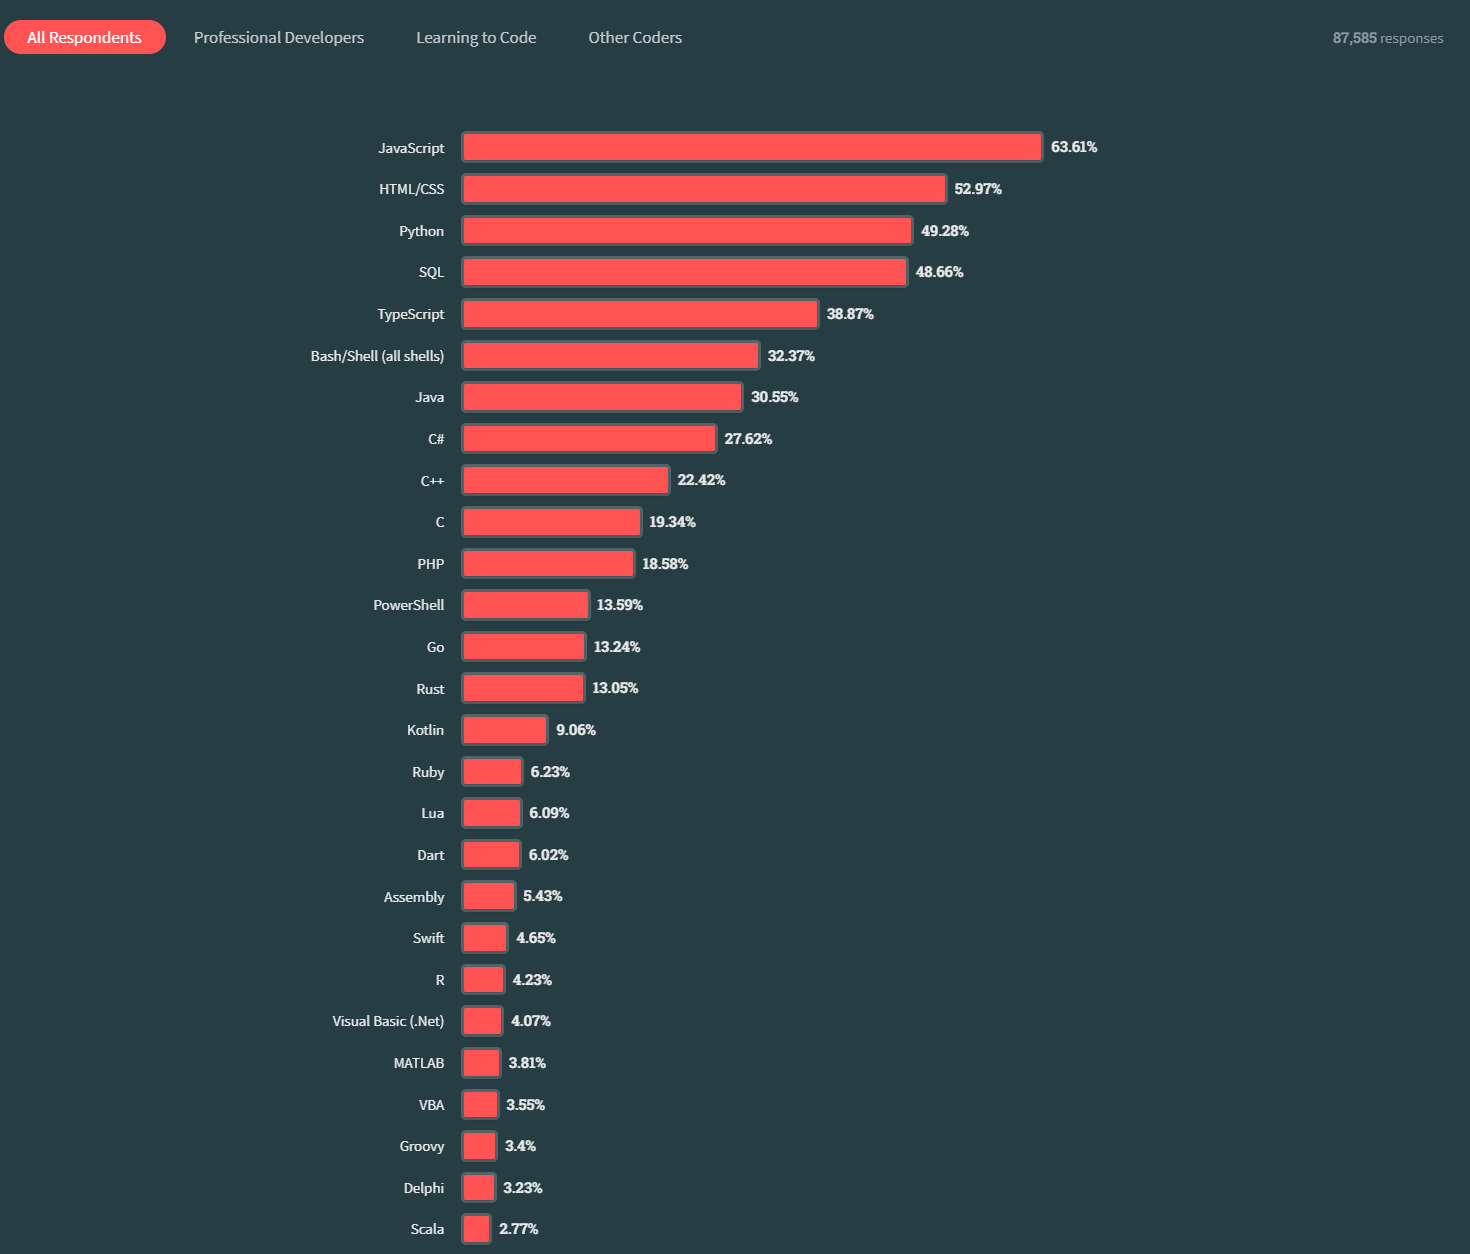
\includegraphics[width=15cm]{images/extrait_sondage_stackoverflow_languages.PNG}
        %légende
        \caption{Capture d'écran d'un diagramme représentant le pourcentage des réponses par langages}
        %label
        \label{fig:StackoverflowLanguages}
    \end{figure}

\subsection{Frameworks utilisés par les sondé.e.s cette année et ceux envisagés pour l'année suivante}

\begin{quote}
    Sur quels \textit{framework} et quelles technologies web avez-vous effectué un travail de développement important au cours de la dernière année, et lesquels souhaitez-vous utiliser au cours de l'année à venir ? (Si vous avez à la fois travaillé avec le cadre et que vous souhaitez continuer à le faire, veuillez cocher les deux cases dans cette ligne.)\footnote{\textit{Which web frameworks and web technologies have you done extensive development work in over the past year, and which do you want to work in over the next year? (If you both worked with the framework and want to continue to do so, please check both boxes in that row.)}}
\end{quote}

\begin{figure}[H]
    %centrer l'image
        \centering
        %commande qui permet de charger une image
        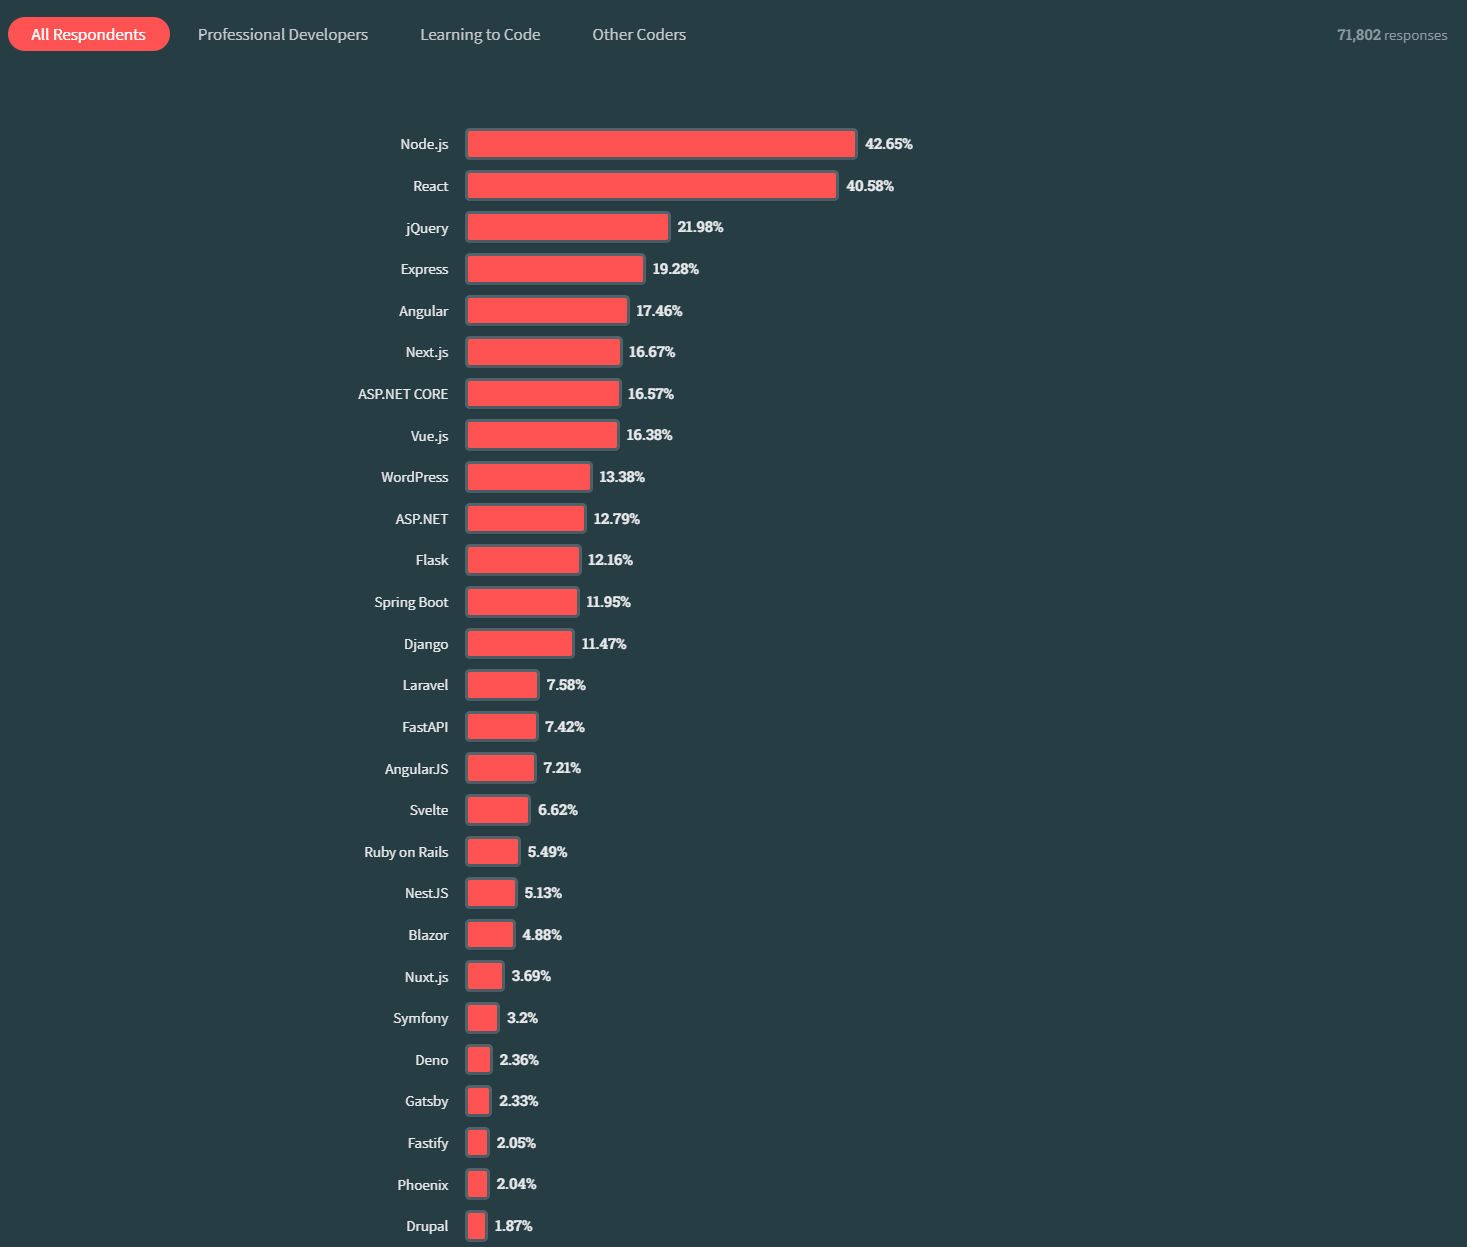
\includegraphics[width=15cm]{images/extrait_sondage_stackoverflow_framework.PNG}
        %légende
        \caption{Capture d'écran d'un diagramme représentant le pourcentage des réponses par frameworks}
        %label
        \label{fig:StackoverflowFrameworks}
\end{figure}


\section{Évolution de l'utilisation du langage Ruby}

\begin{figure}[H]
    %centrer l'image
        \centering
        %commande qui permet de charger une image
        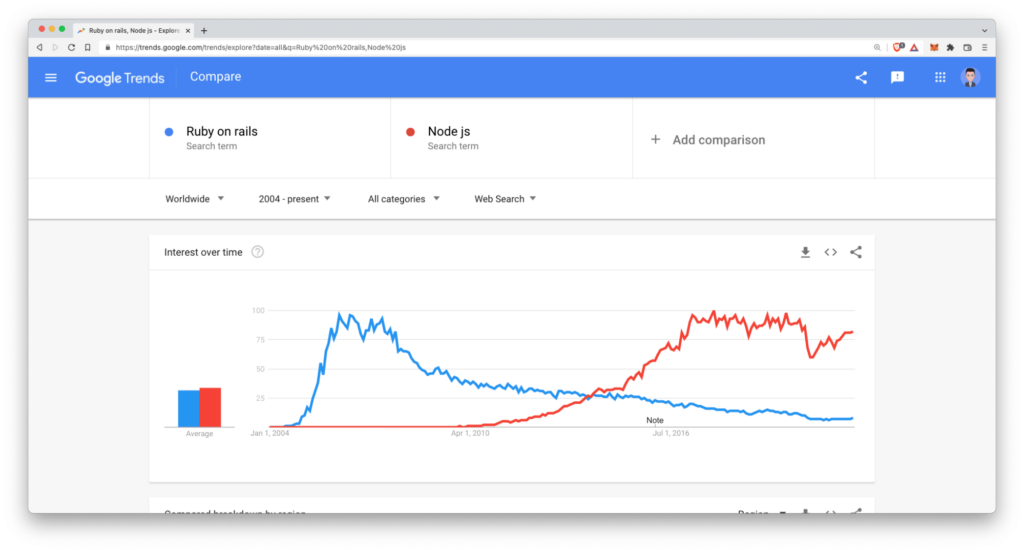
\includegraphics[width=15cm]{images/google-trends-ruby-vs-node.png}
        %légende
        \caption{Capture d'écran comparaison de l'intérêt pour Ruby et pour Node js entre 2004 à aujourd'hui sur Google Trends}
        %label
        \label{fig:RubyvsNodejs}
\end{figure}

\begin{figure}[H]
    %centrer l'image
        \centering
        %commande qui permet de charger une image
        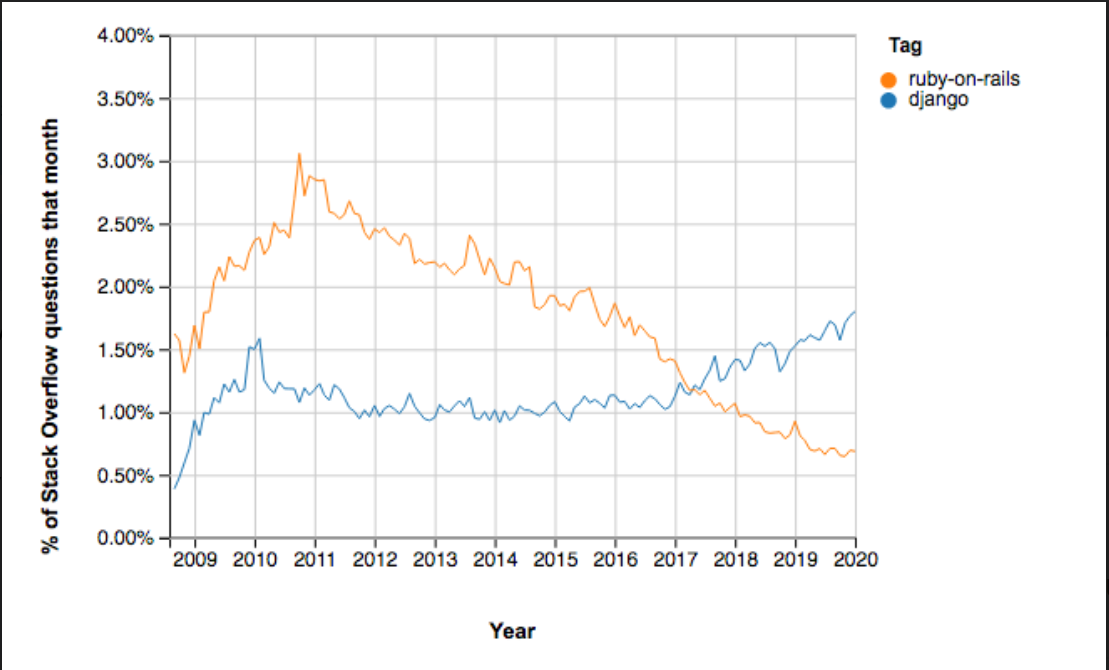
\includegraphics[width=15cm]{images/Ruby_vs_Django_trend.png}
        %légende
        \caption{Capture d'écran comparaison de l'intérêt pour Ruby et pour Django entre 2004 à 2020 sur Google Trends}
        %label
        \label{fig:RubyvsDjango}
\end{figure}


